%% ID: falling_chain
%% TITLE: A Falling Chain
%% TYPE: question
%% QUESTIONTYPE: symbolic
%% CONCEPTS: energy, momentum, eq_of_motion_diff, newtonii
%% VIDEOS: 
%% LEVEL: 5
%% TOPIC: mechanics/dynamics
%% ORDER: 7

\begin{problem}[HE+_Chain] 
{\begin{enumerate}
\item A long chain, with mass per unit length \valuedef{\lambda}{1}{kg\,m\sup{-1}}, is suspended vertically above a table by one end. The chain is allowed to fall, but held so that it always falls at \valuedef{v}{5}{m\,s\sup{-1}}. After \valuedef{t}{5}{s} what is the force exerted downwards on the table?
\item Now a chain with length \valuedef{l}{5}{m} is held above a table by one end, then allowed to fall freely under gravity. The moment the last piece of the chain touches the table, what is the total force being exerted on the table?
\end{enumerate}
}
{\stress{Used with permission from HE+.}}
{\begin{enumerate}
	\item A diagram will help in considering the problem, as in Figure \ref{fig:Dynamics_falling_chain_force}. The chain collects on the ground, to form a mass \vari{M} illustrated in the diagram. The force is then the total mass that has already hit the table, plus the force from the momentum change as the chain comes to rest: \valuedef{\vtr{F}}{\frac{\d \vtr{p}}{\d t}}{}.

\begin{figure}[h]
	\centering
	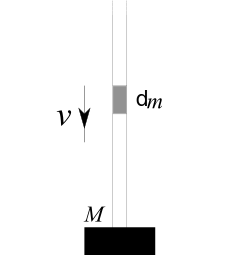
\includegraphics[width=0.3\textwidth]{../../../figures/Dynamics_falling_chain_force.svg}
	\caption{}
	\label{fig:Dynamics_falling_chain_force}
\end{figure}

The total mass that has landed on the table is \valuedef{M}{\int \d m}{} for the time period in question. To relate \vari{\d m} to \vari{\d t}, consider the mass element of the chain; it has mass per unit length \vari{\lambda} and a length \vari{v \d t} lands on the table in a time \vari{\d t}. Thus the mass element is \valuedef{\d m}{\lambda v \d t}{} and so \valuedef{M}{\int_{0}^{t}\lambda v \d t}{}.
\begin{equation*} 
M = \int_{0}^{t}\lambda v \d t = \lambda v t
\end{equation*}
which, since v is constant, could have been found without integration at all. The force from this mass is \vari{F_{M}} $=$ \valuedef{Mg}{\lambda v g t}{}.

The force from the momentum, given by Newton's Second Law, requires us to know \vari{\frac{\d p}{\d t}}. We know \vari{\d m} and so at constant \vari{v}, \vari{\d p} $=$ \valuedef{v \d m}{\lambda v^{2} \d t}{}. Thus \vari{F_{p}} $=$ \valuedef{\frac{\d p}{\d t}}{\lambda v^{2}}{} downwards.

The total force is the sum of \vari{F_{M}} and \vari{F_{p}}:
\begin{eqnarray*} 
F &= F_{M} + F_{p} \\ 
&= \lambda v g t + \lambda v^{2} \\ 
\\ 
&= [(1)(5)(9.8)(5) + (1)(5)^{2}] \\ &= \mbox{\quantity{270}{N}}
 \end{eqnarray*}
	\item When the chain is of length \vari{l} and falling freely under gravity, the situation changes. Since the question only asks about the moment the last link hits the table, however, it becomes somewhat simpler. The mass \vari{M} is now simply the total mass of the chain, and all we need to do is find \vari{v} at the instant the end of the chain hits the table. Conserving energy for the small element at the end of the chain, which feels no force other than gravity because the whole chain moves from rest (i.e. the tension is zero), we find the initial gravitational potential energy has gone into kinetic energy:
\begin{eqnarray*} 
(\d m)gl &= \frac{1}{2}(\d m)v^{2} \\ 
v^{2} &= 2gl 
\end{eqnarray*}
which can be substituted into the expression for \vari{F_{p}} obtained before to find the total force:
\begin{eqnarray*} F &= F_{M} + F_{p} \\ 
&= l\lambda g + \lambda v^{2} \\ 
&= l\lambda g + \lambda (2lg) \\ &= 3 l \lambda g = 3Mg \\ \\ 
&= 3(5)(1)(9.8)
\\ &= \mbox{\quantity{147}{N}}
 \end{eqnarray*}
The total force of the chain as the end hits the table is three times the total mass of the chain.
\end{enumerate}
}
\end{problem}